\section{Related work}

\subsection{General RL Framework}

Reinforcement Learning is most of all a constant interaction between an \emph{Agent}, and an \emph{Environement}. The agent can observe the environement and act at all time. The environement is always evolving and can give \emph{rewards} to the agent depending on the current state and the action performed by the agent. The goal of the agent is to learn and find the best actions to perform in order to maximize the reward obtained.

More formally, we consider a sequence of discrete time steps $t = 1,2,\dots$. At each timestep, the Agent will observe the environement state $x_t$. It will choose to perform an action $a_t$. The agent will receive the reward $r_t$ and the environement will evolve to state $x_{t+1}$. The sequence $x_0, a_0, r_0, x_1, a_1, r_1, \dots$ is called \emph{trajectory}

\begin{figure}[!ht]
    \centering
    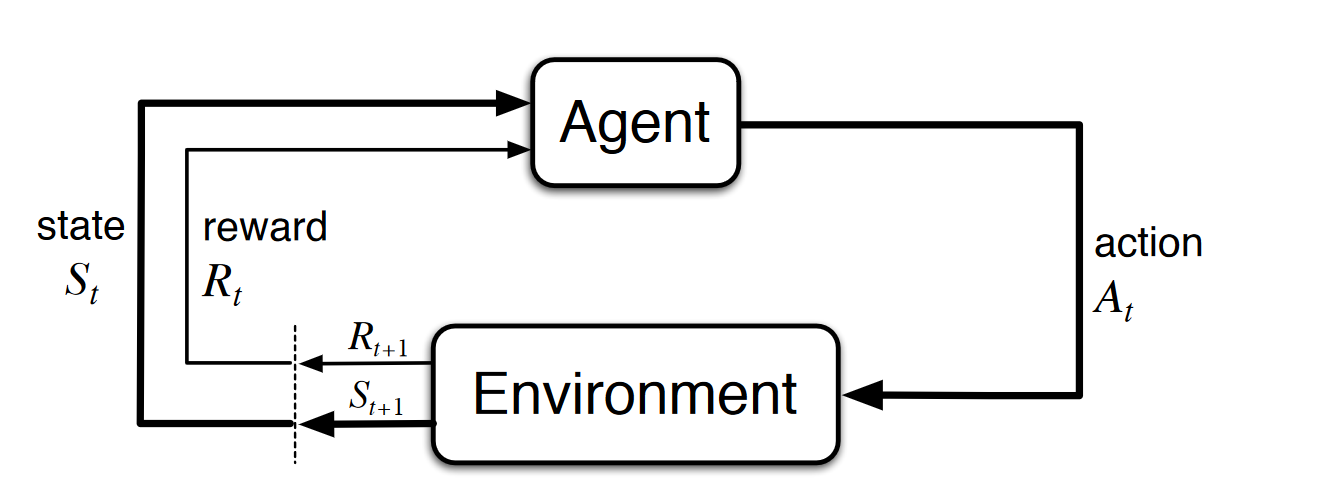
\includegraphics[height=0.2\textheight]{figures/personal_work/MDP.png}
    \caption{The agent-environement interaction\cite{sutton2018reinforcement}}
\end{figure}

In this report we will only consider the Framework of Countable MDPs and the discounted total reward criterion.
We will first start by introducing the general framework of Markov Decision Process (MPD) and the basic results on dynamic programming.

\subsubsection*{Markov Decision Process}

\begin{definition}[Markov Decision Processes \cite{szepesvari2010algorithms}]
An MPD is a tuple $\MM(\XX, \AAA, P, \gamma)$, where:
\begin{itemize}
    \item $\XX$ is a finite state space
    \item $\AAA$ a finite action space
    \item $P$ a transition probability kernel that assigns to each pair $(x,a) \in \XX \times \AAA$ a probability measure on $\XX \times \RR$
    \item $\gamma \in [0,1[$ the discount
\end{itemize}

\end{definition}

The transition probability kernel $P$ works as follow: consider a state $x$ and an action $a$, $P$ gives the probabilities to the next states and the reward received at this timestep, denoted by $P(\cdot |x,a)$. In what follows, we will write $p(x\prime|x, a) = P(\{x\} \times \RR|x,a)$ (resp. $p(x\prime, r|x,a) = P(\{x\} \times r|x,a)$) the probability to reach state $x\prime$ (resp. and receiving reward $r$) when performing action $a$ in state $x$. We also also define the random reward function $r$ so that $r(x,a)$ gives a realisation of reward obtained following $P(\cdot |x,a)$. This reward will be considered bounded almost surely. It is important to notice that the probability to reach the next depends solely on the current state and the current action. What has happened before has no influence, it is the \emph{Markov property}, that is always assumed is this Framework.

\begin{figure}[!ht]
    \centering
    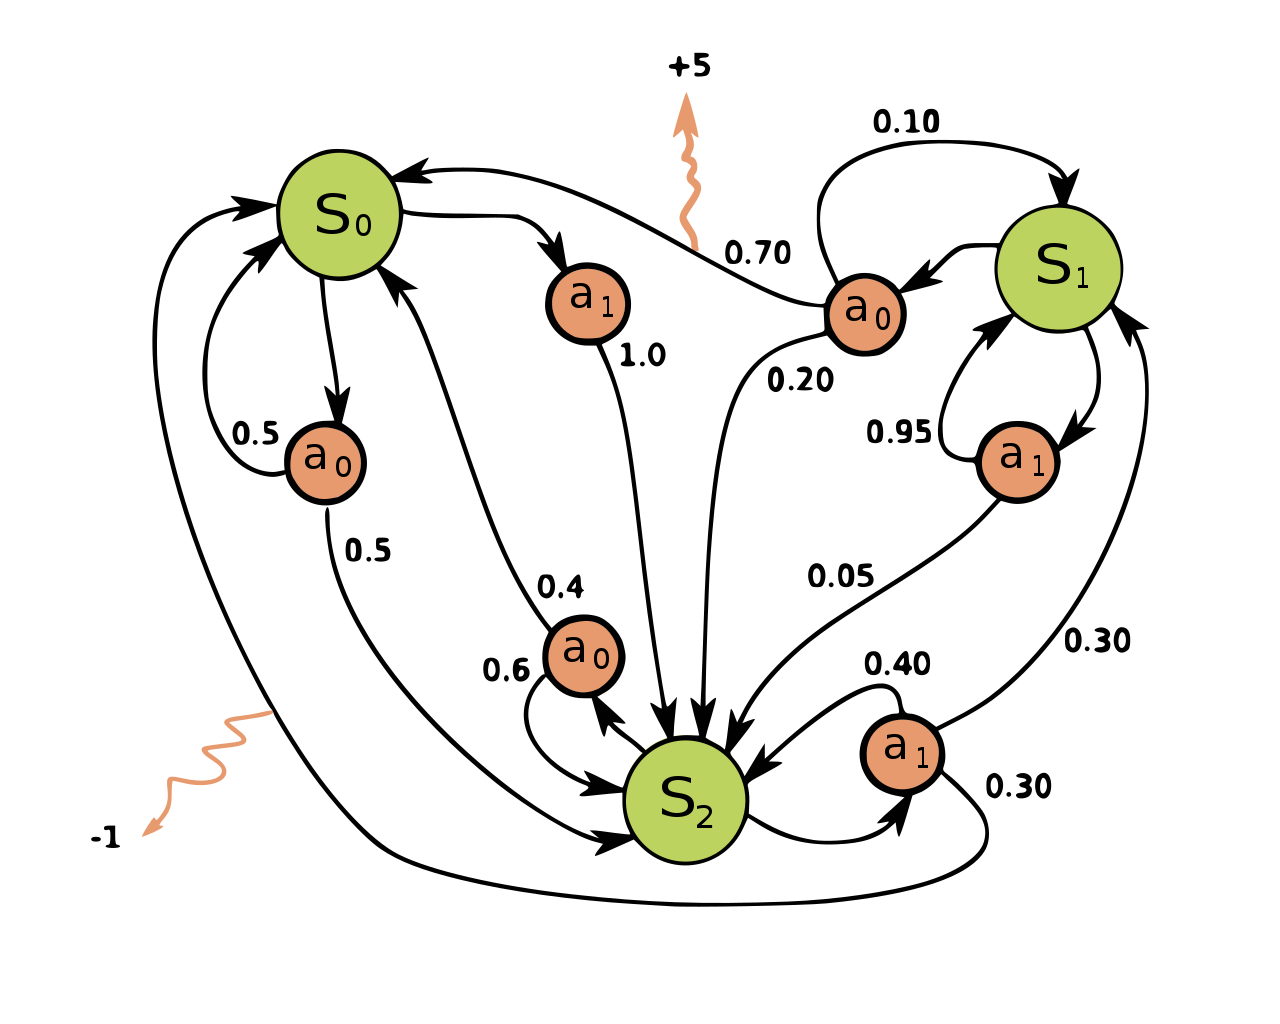
\includegraphics[height=0.3\textheight]{figures/personal_work/Markov_Decision_Process.svg.png}
    \caption{An exemple of MDP\cite{enwiki:1106395391}}
\end{figure}

The MDPs gives the formalisation of an environnent, we then need to formalize what it means for the agent to learn. We already defined a reward, that we said we wanted to maximise. However, the sequence of reward $r_0, r_1, r_2, \dots$ is random, the question is what do we maximise on this sequence. What is usually done, and what we will consider here, is to consider the sum of rewards, called the \emph{Return}:

\[ \mathcal{R} = r(x_0, a_0) + r(x_1, a_1) + \dots \]

There are two issues that arise with this definition, making it not really well defined. The first is the return being random, which is dealt with by considering the \emph{mean} of the return, giving the \emph{expected return}. The second is that, even with the expected return, we only assumed the reward to be bounded, so that return may not always be finite. This is where the discount $\gamma$ from the definition of the MDP comes to play: we consider the \emph{Discounted Expected Return} (later called simply "Return"). The goal of the agent will be to maximize this precise quantity:

\[ R = \EE{ r(x_0, a_0) + \gamma r(x_1, a_1) + \gamma^2 r(x_2, a_2) +  \dots} = \EE{\sum_{t=0}^\infty  \gamma^t r(x_t, a_t)} \]

It is now well defined and bounded: if $M$ is a bound on the reward almost surely, then :

\begin{align*}
    |R| = \left|\EE{\sum_{t=0}^\infty  \gamma^t r(x_t, a_t)}\right|& \leq \sum_{t=0} ^\infty  \gamma^t M \leq \frac{1}{1-\gamma}M
\end{align*}

The discount is important to make the sum converging, but it also has some practical implications. Because of how it is defined, the later the reward is obtained, the less worth it is. The same reward received $k$ step later is considered $\gamma^{k}$ less. Implicity, it encourages the agent to get this reward as soon as possible, to accomplish a certain task quicker. This choice is quite arbitrary but leads to a rich theory because of its computational properties and ease to manipulate.\\

We also need to emphasize on the choice of the mean. While it is a quite intuitive choice to make here and will also lead to a rich theory, it reduces greatly the information on all the possiblities, and doesn’t really take into account what happens in the extreme cases. It will require the study of the so-called "risk-sensitive" Reinforcement Learning.

\subsubsection*{Policies and value functions}

We have a formalization of the environment and a quantity we want to optimize through actions. Before dwelling in the first results of the theory, we last need to formalize the choice of actions of the agent. For that we introduce \emph{decision rules} and \emph{policies}. 

\begin{definition}
    A decisision rule $d$ is a function that maps each state to a probability distribution on the action space :
    
    \[ d: \XX \mapsto \PPPP(\AAA) \]

    It is said \emph{deterministic} if it of the form d: $\XX \mapsto \AAA$ \\
\end{definition}

\begin{definition}
    A policy is a sequence of decision rule: 

    \[ \pi = (d_0, d_1, d_2, \dots) \]

    It is said \emph{stationnary} if it uses a unique decision rule.
\end{definition}

When exploring the environement, the agent will use a policy to choose its action. It works as follows: at each time step $t$, the agent will perform an action $a$ sampled from $\pi(\cdot | x_t)$, which will lead to a reward and a next state sampled from $P(\cdot |x,a)$, then the policy gives another action, and so on.

To be able to evaluate each policies, we define the \emph{value functions}:

\begin{definition}
    The Value function $V$ is defined by:
    \[ V^\pi(x) = \EE{\sum_{t=0}^\infty  \gamma^t r(x_t, a_t) | x_0 = x}  \]
    with $x_t \sim p(\cdot | x_{t-1}, a_{t-1})$ and $a_t \sim \pi(\cdot | x_t)$
\end{definition}

This value function $V(x)$ simply represents the expected discounted reward received following policy $\pi$ and starting at state $x$. With this definition, we can now formalize the problem of RL as an optimization problem, the problem of finding an \emph{optimal policy}:

\begin{definition}[Optimal Policy]
    An optimal policy is a policy that verifies:

    \[ \sta{\pi} \in \argmax_\pi \ V^\pi(x) \quad \forall x \in \XX \]
\end{definition}

By convenience for the future, we also define the action-state value function :
\begin{definition}
    The  Q-value function (also called action-state value function) is defined by:
    \[ Q^\pi(x,a) = \EE{\sum_{t=0}^\infty  \gamma^t r(x_t, a_t) | x_0 = x, a_0 = a}  \] 
    with $x_t \sim p(\cdot | x_{t-1}, a_{t-1})$ and $a_t \sim \pi(\cdot | x_t)$
\end{definition}

\subsubsection*{A first result on the policies}

Now that the framework have been properly formalized, and before trying to compute the Value function and the optimal policies, this first result will simplify the theory

\begin{definition}[The Discounted Occupancy Measure\cite{bertsekas2012dynamic}]
    Consider the MDP $\MM(\XX, \AAA, P, \gamma)$. We define the \emph{Discounted Occupancy Measure} $p_\gamma^\pi$ by:

    \[ \forall x \in \XX, a \in \AAA, \quad p_\gamma^\pi(x,a) = (1-\gamma)\sum_{t=0}^\infty \gamma^t \PP\left[x_t = x, a_t = a\right] \]

    We then have the following rewriting of the value function:

    \[ V^\pi(x) = \frac{1}{1-\gamma} \sum_{x,a} p_\gamma^\pi(x,a)\EE{r(x,a)} \]
\end{definition}

This new writing of the value function, while seaming a bit more complicated, allows to summarize the influence of the policy in a unique term. It is used in the following results by Bertsekas:
% \begin{proof}
%     \begin{align*}
%         V^\pi(s) &= \EE{\sum_{t=0}^\infty  \gamma^t r(x_t, a_t) | x_0 = x}\\
%         &= \sum_{t=0}^\infty  \gamma^t \EE{ r(x_t, a_t) | x_0 = x}\\
%         &= \sum_{t=0}^\infty  \gamma^t \sum_{x,a} \PP\left[x_t = x, a_t = a | x_0 = x\right]\EE[r(x, a)]\\
%         &= \frac{1}{1-\gamma} \sum_{x,a} (1-\gamma) \sum_{t=0}^\infty \PP\left[x_t = x, a_t = a | x_0 = x\right]\EE[r(x, a)]\\
%         &= \frac{1}{1-\gamma} \sum_{x,a} p_\gamma^pi(x,a)\EE[r(x,a)]
%     \end{align*}
   
% \end{proof}
\begin{theorem}[Bertsekas, 2007]
    Consider a MDP $\MM(\XX, \AAA, P, \gamma)$ with the previous assumptions. For any \emph{non-stationnary policy} $\pi$, there exists a \emph{stationnary policy} $\bar{\pi}$ such that 

    \[ \forall x\in \XX, a \in \AAA, \quad p_\gamma^{\bar{\pi}}(x,a) = p_\gamma^{\pi}(x,a) \]
\end{theorem}

Combined with the rewriting of the value function, this mean that for any value function obtainend with a non-stationary policy, we can obtain the same with a stationary one. 

\begin{corollary}
    If an optimal policy exists, then the optimal policy can be choosen to be stationnary.
\end{corollary}

We can now restrain ourself to stationary policy when studying the theory further. From now on, except mentioned otherwised, all policies will be assumed to be stationary.

\subsection{Dynamic Programming}

\subsubsection*{Policy Evaluation} 

The first problem when considering a policy, is to evaluate it, \ie compute the Value function. The issue with its definition, being a mean on a infinite sum of random variables, makes significantly hard to compute directly as it is. Fortunately by using the linearity of the mean and the infinite sum, we find that the value function (and the Q-value function) verifies a recursive formula, called \emph{Bellman Equation}

\begin{align*}
V^\pi(x) &= \sum_{a \in \AAA} \pi(a|x) \left( \EE{r(x,a)} + \gamma \sum_{x^\prime  \in \XX} p(x^\prime |x,a)V^\pi(x^\prime ) \right) \\
Q^\pi(x,a) &= \EE{r(x,a)} + \gamma \sum_{x^\prime ,a^\prime  \in \XX \times \AAA} p(x^\prime |x,a)\pi(a^\prime |x^\prime )Q^\pi(x^\prime ,a^\prime )
\end{align*}

Those equations give a linear system of equation, with as many constraints as unknown ($|\XX|$ for the value function, $|\XX||\AAA|$ for the Q-value function). Which means it can be solved through matrix inversion: with $V^\pi \in \RR^{|\XX|}, r^\pi \in \RR^{|\XX|}, P\pi \in \RR^{|\XX|\times \XX},$

\begin{align*}
    V^\pi = r^\pi + \gamma P^\pi V^\pi \Longrightarrow V^\pi =  \left(I - \gamma P^\pi\right)^{-1}r^\pi
\end{align*}

This is very useful to compute the exact values in small instances, but there is another way to compute it, by iteration. For that, we will need to introduce the \emph{Bellman Operator}

\begin{definition}[Bellman Operator]
Let $V: \XX \mapsto \RR$ or $Q: \XX \times \AAA \mapsto \RR$, $\pi$ a policy. The Bellman operator $\TT^\pi$ is defined by:
\[ \forall x \in \XX, \qquad \TT^\pi V(x) = \sum_{a \in \AAA} \pi(a|x) \left( \EE{r(x,a)} + \gamma \sum_{x^\prime  \in \XX} p(x^\prime |x,a)V(x^\prime ) \right) \]
\[ \forall x,a \in \XX \times \AAA, \qquad \TT^\pi Q(x,a) = \EE{r(x,a)} + \gamma \sum_{x^\prime ,a^\prime  \in \XX \times \AAA} p(x^\prime |x,a)\pi(a^\prime |x^\prime )Q(x^\prime ,a^\prime ) \]
\end{definition}

Those operators are directly linked to the Bellman equation, which can be rewrited simpler this way :

\begin{align*}
    \TT^\pi V^\pi(x) &=  V^\pi(x)  \\
    \TT^\pi Q^\pi(x,a) &= Q^\pi(x,a) 
\end{align*}

From this we get that the value functions are fixed points of the Bellman Operators. Fixed points are essential in mathematics are allow for, under the right assumptions, for computation or proof or existence of object hard to handle. Most of it comes from the following result:

\begin{theorem}[Banach fixed point\cite{rudin1991functional}]
Let $( X , d )$ be a non-empty complete metric space with a contraction mapping $ T : X \mapsto X$. Then $T$ has admits a unique fixed-point $\sta x\in X$ and
\[ \forall x \in X, \quad T^n(x) \longrightarrow \sta x \text{ exponentially} \]
\end{theorem}

The theorem is applicable here because we get the following property:

\begin{proposition}
    The bellman operators are a $\gamma$--contractions:

    \begin{align*}
        \forall V_1, V_2 \in \RR^{|\XX|}, \quad &|| \TT^\pi V_1 - \TT^\pi V_2 ||_\infty \leq \gamma ||  V_1 - V_2 ||_\infty\\
        \forall Q_1, Q_2 \in \RR^{|\XX|\times \AAA}, \quad &|| \TT^\pi Q_1 - \TT^\pi Q_2 ||_\infty \leq \gamma ||  Q_1 - Q_2 ||_\infty
    \end{align*}
\end{proposition}

The fixed point algorithm thus gives a very simple iteration algorithm to get the value function, called \emph{Value Evaluation}: apply the Bellman Operator up to convergence with any starting values, up to a choosen point of convergence.

This algorithm will also give rise to 2 iteration algorithms to find optimal policies in a MPD.

\subsubsection*{Control} 

The second and main problem in Reinforcement Learning is to find a policy that maximizes the expected return. We to do so, the strategy will be quite similar to how we got to an algorithm for policy evaluation. First, we start by introducing the \emph{Optimal Value functions}

\begin{definition}
    The optimal value function are defined by:

\begin{align*}
\sta V(x) &= \max_{\pi} \EE{\sum_{t=0}^\infty  \gamma^t r(x_t, a_t) | x_0 = x} = V^{\sta\pi}(x)\\
\sta Q(x,a) &= \max_{\pi} \EE{\sum_{t=0}^\infty  \gamma^t r(x_t, a_t) | x_0 = x, a_0 = a} = Q^{\sta\pi} (x,a)
\end{align*}
\end{definition}

The definition of those functions can also be derived to show that they verify a recursive equation. Those one are called \emph{Bellman Optimality Equations}:
\begin{align*}
\sta V(x) & = \max_{a \in \AAA} \EE{r(x,a)} + \gamma \sum_{x^\prime  \in \XX} p(x^\prime |x,a)\sta V(x^\prime ) \\
\sta Q(x,a) & = \EE{r(x,a)} + \gamma \sum_{x^\prime  \in \XX} p(x^\prime |x,a)\max_{a^\prime  \in \AAA}\sta Q(x^\prime ,a^\prime )
\end{align*}
This equation is important not only for defining operators, but also because it leads to another theoretical results on policy. By looking at it, we notice that an optimal policy takes the action that maximizes the value function of the next state. An optimal policy can thus be chosen deterministic: this is the \emph{Bellman optimality principle}

\begin{proposition}[Bellman optimality principle\cite{bellman1966dynamic}]
    An optimal policy has the property that whatever the initial state and initial decision are, the remaining decisions must constitute an optimal policy with regard to the state resulting from the first decision
\end{proposition}

\begin{corollary}
    If an optimal policy exists, then it can be chosen to be deterministic.
\end{corollary}

Combining with the previous result on policies, although we started with very general policies, we find that the theory can be reduced to only using stationary and deterministic ones. This a specificity of the framework with the different choice that were, such as optimizing on a mean of a discounted return. We will see later that it may not be so easy in a different framework.\\

The previous results also suggests that there would only be $|\XX||\AAA|$ policies to check, but evaluating and checking them all is still quite costly. Instead, we will proceed by introducing an optimal version of the Bellman Operator, adapted to the Optimal Value Functions.

\begin{definition}[Optimal Bellman Operator]
Let $V: \XX \mapsto \RR$ or $Q: \XX \times \AAA \mapsto \RR$, $\pi$ a policy. The Bellman operator $\sta \TT$ is defined by:
\[ \forall x \in \XX, \qquad \sta\TT V(x) = \max_{a \in \AAA} \EE{r(x,a)} + \gamma \sum_{x^\prime  \in \XX} p(x^\prime |x,a)\sta V(x^\prime ) \]
\[ \forall x,a \in \XX \times \AAA, \qquad \sta \TT Q(x,a) = \EE{r(x,a)} + \gamma \sum_{x^\prime  \in \XX} p(x^\prime |x,a)\max_{a^\prime  \in \AAA}\sta Q(x^\prime ,a^\prime ) \]
\end{definition}

These operators happen to verify the same contraction properties as the previous case:

\begin{proposition}
    The optimal bellman operators are a $\gamma$--contractions:

    \begin{align*}
        \forall V_1, V_2 \in \RR^{|\XX|}, \quad &|| \TT V_1 - \TT V_2 ||_\infty \leq \gamma ||  V_1 - V_2 ||_\infty\\
        \forall Q_1, Q_2 \in \RR^{|\XX|\times \AAA}, \quad &|| \TT Q_1 - \TT Q_2 ||_\infty \leq \gamma ||  Q_1 - Q_2 ||_\infty
    \end{align*}
\end{proposition}

We can now deduce an iterative algorith, called \emph{Value iteration}: apply the Bellman Operator up to convergence with any starting values, up to a choosen point of convergence.
































% \newpage
% \subsection{unformal Distributional Approach (with random variable)[TO REMOVE]}

% \paragraph{Policy Evaluation:} 

% We here want to look at the full distribution of the return when following a certain policy $\pi$. We define the random return as follow (recall that $R$ is a stochastic reward):

% \begin{definition}[Value distribution function]
% The random value function associated with policy $\pi$ is defined as follow:
% \[ \VV^\pi(x) = \sum_{t=0}^\infty  \gamma^t R(x_t, a_t) \qquad x_0 = x \]
% \[ \QQQ^\pi(x,a) = \sum_{t=0}^\infty  \gamma^t R(x_t, a_t) \qquad x_0 = x, a_0 = a \] 
% with $x_t \sim p(\cdot | x_{t-1}, a_{t-1})$ and $a_t \sim \pi(\cdot | x_t)$
% \end{definition}

% By doing the same computation as in the expected reward case, we notice that the value distribution functions verifies an extended version of the Bellman equation:

% \begin{align}
% \VV^\pi(x) & = \sum_{a \in \AAA} \pi(a|x) \left( R(x,a) + \gamma \sum_{x^\prime  \in \XX} p(x^\prime |x,a)\VV^\pi(x^\prime ) \right) \\
% \QQQ^\pi(x,a) & = R(x,a) + \gamma \sum_{x^\prime ,a^\prime  \in \XX \times \AAA} p(x^\prime |x,a)\pi(a^\prime |x^\prime )\QQQ^\pi(x^\prime ,a^\prime )
% \end{align}

% This leads to the distributional Bellman operator:

% \begin{definition}[Distributional Bellman Operator]
% \[ \forall x \in \XX, \qquad \TT^\pi \VV(x) = \sum_{a \in \AAA} \pi(a|x) \left( R(x,a) + \gamma \sum_{x^\prime  \in \XX} p(x^\prime |x,a)\VV(x^\prime ) \right) \]
% \[ \forall x,a \in \XX \times \AAA, \qquad \TT^\pi \QQQ(x,a) = R(x,a) + \gamma \sum_{x^\prime ,a^\prime  \in \XX \times \AAA} p(x^\prime |x,a)\pi(a^\prime |x^\prime )\QQQ(x^\prime ,a^\prime ) \]
% \end{definition}

% Due to the distribution persepective, it is not possible to solve for the fixed point equation with a matrix inversion anymore. But the following result still enable theoretical computation of the exact random value distribution:

% \begin{lemma}
%     $\TT$ is a $gamma$-contraction in $d_p$
% \end{lemma}

% leads to an algorithm to find the compute the distribution

% \paragraph{Control:}

% \begin{definition}[Optimal Value distribution function]
%     \[ \sta \VV \in \{\VV^{\sta\pi} \in \argmax_\pi \EE{\VV^\pi}\} \]
%     \[ \sta \QQQ \in \{\QQQ^{\sta\pi} \in \argmax_\pi \EE{\QQQ^\pi}\} \]  
% \end{definition}

% This distribution also verify an extended version of the Optimal Bellman Equation:

% \[ \sta \VV(x) =  R(x,\sta a(x)) + \gamma \sum_{x^\prime  \in \XX} p(x^\prime |x,\sta a(x))\sta V(x^\prime ) \]
% \[ \sta \QQQ(x,a) = R(x,a) + \gamma \sum_{x^\prime  \in \XX} p(x^\prime |x,a)\sta Q(x^\prime ,\sta a(x)) \]

% and leads to the optimal bellman operator:

% \begin{definition}[Optimal Distributional Bellman Operator]
%     \[ \forall x \in \XX, \qquad \sta\TT \VV(x) = R(x,\sta a(x)) + \gamma \sum_{x^\prime  \in \XX} p(x^\prime |x,\sta a(x)) V(x^\prime ) \]
%     \[ \forall x,a \in \XX \times \AAA, \qquad \sta \TT \QQQ(x,a) = R(x,a) + \gamma \sum_{x^\prime  \in \XX} p(x^\prime |x,a) Q(x^\prime ,\sta a(x)) \]
% \end{definition}

% However, this operator is not a contraction (see Bellemare 2017). But we still have some practical theoretical results: contraction in mean. Also, convergence in sequence of optimal policy (details ?)